\section{Le diagramme de classes}
Pour la cr�ation du diagramme de classes, l'id�e est de regrouper les
diff�rents paquetages qui s'utilisent de fa�on identique. Les
paquetages compte et droit a �t� cr�� pour g�rer les droits
d'identification et d'acc�s des diff�rents acteurs.
Dans ce diagramme nous avons les objets:\\

\begin{itemize}
\item Account:
C'est un objet qui identifie un utilisateur par son login et son mot
de passe. C'est l'objet de base du paquetage compte. Seul
l'administrateur a le droit de le modifier ou de le supprimer.\\

\item AccountManager:
C'est le g�rant des comptes et c'est lui qui re�oit la requ�te d'un
utilisateur qui veut se loger.
Il utilise les param�tres du compte de l'utilisateur pour v�rifier la
validit� de ces derniers avant de le connecter � l'application.
Cette v�rification se fait par d�l�gation de la requ�te du
consultant � l'objet AccountData.\\

\item AccountData:
C'est l'objet qui stocke les informations sur les comptes des utilisateurs.
C'est lui qui v�rifie la validit� d'un compte.\\

\item RigthManager:
C'est un objet qui permet � l'administrateur ou au responsable de
pouvoir rechercher ou modifier les droits � un enseignant.\\
\end{itemize}


\begin{center}
\scalebox{0.4}{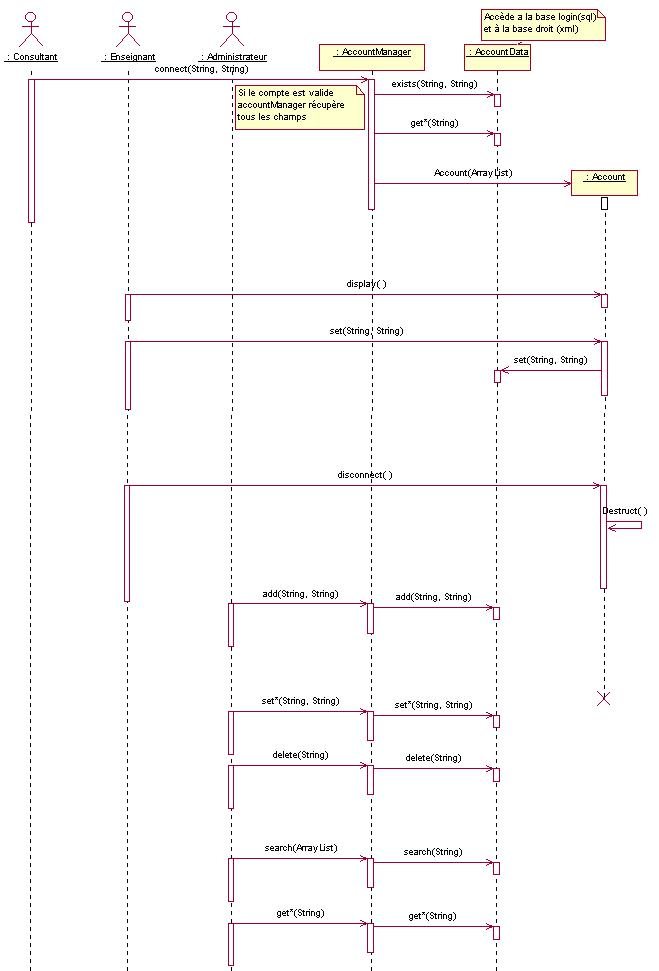
\includegraphics{images/compte.jpg}}\\
\end{center}







